\documentclass[12pt, letterpaper, fleqn]{report}
\usepackage[hidelinks]{hyperref}
\usepackage{geometry}
\usepackage{graphicx}
\usepackage{fix-cm}

\geometry{letterpaper, total={210mm,297mm}, left=20mm, right=20mm, top=20mm, bottom=20mm}

% Font size convention for this document:

% UI element : \textsl{name of the UI element}
% Nomenclature: ``name of the term defined''

\begin{document}

\begin{titlepage}
\begin{center}

% http://www.tex.ac.uk/cgi-bin/texfaq2html?label=fontsize
\textbf{\textsc{\fontfamily{phv}\fontsize{30}{36}\selectfont User Manual}}\\[1.0cm]
\textbf{\textsc{\fontfamily{phv}\fontsize{30}{36}\selectfont AND}}\\[1.0cm]
\textbf{\textsc{\fontfamily{phv}\fontsize{30}{36}\selectfont TECHNICAL DOCUMENTATION}}\\[1.0cm]
\textbf{\textsc{\fontfamily{phv}\fontsize{30}{36}\selectfont FOR}}\\


\includegraphics[width=1\textwidth]{WHAT_banner}~\\[1cm]

\end{center}
\end{titlepage}


\chapter*{License}

WHAT is free software: you can redistribute it and/or modify it under the terms of the GNU General Public License as published by the Free Software Foundation, either version 3 of the License, or (at your option) any later version.

This program is distributed in the hope that it will be useful, but WITHOUT ANY WARRANTY; without even the implied warranty of MERCHANTABILITY or FITNESS FOR A PARTICULAR PURPOSE. See the GNU General Public License for more details.

You should have received a copy of the GNU General Public License along with this program. If not, see \url{www.gnu.org/licenses}.

\newpage

\chapter*{Acknowledgements}

WHAT has been funded in part by:

\begin{description}
\item{CRSNG through a PhD grant to Jean-Sébastien Gosselin}
\item{Projet Montérégie Est PACES}
\item{CRSNG fund}
\item{CGC}
\end{description}

We would like to thank all people who have used WHAT since its earliest stages and provided essential technical feedback, constructive criticism, and helpful comments or have helped in the shaping of the science that lies under the hood of the software. In particular, special thanks to (in alphabetical order):

\begin{description}
\item{Erwan Gloaguen, Professor of Geophysics and Geostatistics, INRS-ETE, Quebec, QC, Canada.}
\item{Harold Vigneault, Research Professional, INRS-ETE, Quebec, QC, Canada.}
\item{Marc Laurencelle, PhD Student in Earth Sciences, INRS-ETE, Quebec, QC, Canada.}
\item{Pierre Ladevèze, PhD Student in Earth Sciences, INRS-ETE, Quebec, QC, Canada.}
\item{René Lefebvre, Professor in Hydrogeology, INRS-ETE, Quebec, QC, Canada.}
\item{Xavier Mallet, Research Technician, Geological Survey of Canada – Quebec Division, QC, Canada.}
\end{description}

\newpage

\chapter*{Introduction}

WHAT (Well Hydrograph Analysis Toolbox) is a free, open source, and cross-platform interactive computer program whose main focus is the interpretation of observation well hydrographs, including:

\begin{itemize}
\item{the preparation of a gapless daily weather time-series (precipitation and air temperature) representative of the well location. For this purpose, an interface to the online Canadian Daily Climate Database (CDCD) is provided that allows to query stations interactively by location coordinates, download the available data, and automatically rearranged the data in a format compatible with WHAT. Furthermore, missing data for a given station can be quickly filled with data from selected neighboring weather stations using a multiple linear regression model;}
\item{the generation of various publication-quality figures from the weather and water level data;}
\item{the exploration, manipulation, and validation of the data within a user-friendly dynamic graphical environment;}
\item{the calculation of the master recession curve of the well hydrograph (experimental);}
\item{the estimation of groundwater recharge at the local scale in unconfined conditions with a method combining the daily meteorological data and the water level time series (will be available in a future release).}
\item{the calculation of the barometric response function of the well that can be used to assess the level of confinement of the aquifer at the well location (will be available in a future release).}
\end{itemize}

WHAT is written in the Python 2.7 programming language and is currently maintained and developed by Jean-Sébastien Gosselin at INRS-ETE (\url{www.ete.inrs.ca}). The source code and a stand-alone executable for Windows 7 are available free of charge for download on GitHub (\url{https://github.com/jnsebgosselin/WHAT}). If you encounter any problems or errors during program execution, have any questions, or have specific suggestions on how to improve WHAT, please contact Jean-Sébastien Gosselin at this email address \href{mailto:jnsebgosselin@gmail.com}{jnsebgosselin@gmail.com}.

\tableofcontents

\listoffigures

\chapter{User Manual}


\section{Installation}\label{sec:intallation}

WHAT can run on Windows, Linux, or OS X computer operating systems. However, a stand-alone executable of the program is currently released and tested only for the Windows 7 platform. This executable should also be compatible with Windows XP. For the Linux and OS X platforms, the software can be run directly from the source code, provided that Python 2.7 and all the required third party packages are installed on the computer (PySide, NumPy, matplotlib, xlrd, xlwt).

The stand-alone executable for Windows 7 is distributed in a Zip archive that can be downloaded freely on GitHub (\url{https://github.com/jnsebgosselin/WHAT/releases}). This archive contains:

\begin{itemize}
\item{the GNU General Public License;}
\item{a folder named WHAT that contains all the necessary system files for the program to run, including the file WHAT.exe from which the software can be started;}
\item{a folder named Projects where all input and output files used or created by WHAT are stored by default. In this folder are included samples of input and output files that provide a quick and convenient way to test and learn the various features of the program.}
\end{itemize}

Once the content of the Zip archive has been extracted, the program can be started directly from the WHAT.exe executable file that is contained withing the folder named WHAT. The software can conveniently run from any location on the computer or from any storage device without the need to install the program beforehand.

\section{Overview of the Graphical User Interface}

WHAT Graphical User Interface (GUI) mainly consists of a menu bar, a console area, and a central view panel (see Figure 1). The menu bar is located in the top right corner of WHAT main window. This is where you can view and edit the current project directory. The project directory is a folder location where all the input, output and parameter files associated with a given project are gathered. For more information about the project directory content and files organization, please refer to section 2.3.2. When opening WHAT for the first time, the current project is setup by default to an example that is provided with the software with the necessary files to test all the functionalities of the program. The console is located at the bottom of the main window and is used to report technical information about the various tasks accomplished by the program as well as warning and error messages. The console can be completely collapsed to save space, or can be fully expanded to the entire area of the window. The central view panel is equipped of a tab bar at the top where you can navigate through the various functionalities of the program. There is a total of four tabs available: Download Data, Fill Data, Hydrograph, and About. The tabs are described in a little bit more details in the text below and are also presented in Figures 2 to 5.

The Download Data tab (Figure 2) provides an interface to the online Canadian Daily Climate Database (CDCD) that allows to query stations interactively by location coordinates, download the available data, and automatically rearranged the data in a format compatible with WHAT. Alternately, it is possible to provide a custom list of Canadian weather stations for which data can be downloaded and formatted. At the moment, it is not possible to access data of weather stations located in the U.S. This feature may be added in a future release of the software.

The Fill tab (see Figure 3) is where you can automatically estimate the missing daily weather values in your data to create gapless time-series of daily precipitation and air temperature. Missing data for a given station are estimated from selected neighboring weather stations using a multiple linear regression model;

The Hydrograph tab is used for viewing and plotting data. For this purpose, two modes are available: the layout and the computation mode. Both modes share the same weather and water level dataset. It is possible to switch from one mode to the other at anytime. The layout mode (see Figure 4) provides an interface to interactively produce publication-quality graphs from the data. The computation mode (see Figure 5) consists in a dynamic graphical environment where data can be explored, manipulated and analyzed. Various computation tools are available in this mode, including the estimation of the hydrograph Master Recession Curve (MRC) and the estimation of groundwater recharge.

The About tab displays copyright, licensing and general information about WHAT.

\section{Interpretation of water-level time-series with WHAT}

\subsection{Introduction}

WHAT essentially consists of set of tools to assist the interpretation of water level time series measured in observation wells, from the preparation of raw data to the assessment of groundwater recharge when in unconfined conditions. In this perspective, WHAT was developed with the general workflow shown in Figure 6  in mind.

The first step consists in the preparation of a gapless weather dataset.

Validation/preparation of water level time series: 1) automatic measurements fitted to manual measurements. 2) Correct the places where there is a break in the water level curve. This is due generally to the logger that is placed at a different level following the removal of the later from the well. 3) Remove measurements that were acquired while the barologger was outside the water column.

Preparation of a gapless weather dataset. This include. Downloading data from the CDCD database for stations located in a radius of 0 to 100 km from the well. Fill missing daily data for the station located closest to the well by using selected neighboring stations. Data are not interpolated to the exact location of the well. It has been decided to keep the original dataset of the station located closest to the well to analyse the data. This is due to the fact that conventional technique for interpoloating weather data tend to surestimate the number of wet day, but underestimate the intensity of stron precipitation event. More advanced and complicated technique are required to circumvent these issues. It has thus been decided that is was prefereable to keep the original data from a single station.

Once the weather data, and water level are prepared, production of a well hydrograph. Visual interpretation between the water level  fluctuation and weather data can be done.

If high time resolution measurement of the water level and barometric pressure are available, it is possible to carry an calculation of the barometric response function. It is also good to produce a FFT analysis of the hydrograph.
Weather yearly average and montlhy averages can be plotted at this stage.
If the visual inspection of the well, and the barometric response function, determined that the well in unconfined, it means groundwater recharge can be estimated from the data. First, determining the segment where groundwater recharge can be supposed to be negligible and where the water level recede. After that, compute the MRC, and compute a first estimation of groundwater recharge using the Water-Table Fluctuation principle. Estimate finaly recharge with a method combining the meteorological data and the well hydrograph. Enjoy.

\subsection{New and Open Project}

Data is managed in WHAT by project. That is all input and output files relative to a given project are saved within a common folder called the ``project folder''. This file management system allows you to easily backup and move your projects from one location to the other since all the files relating to a same project are saved at the same location.

By default, the current active project is setup to an example that is distributed with the software. To start a new project, click on the \textsl{New Project\dots} button located at the right end of the WHAT menu bar (see Figure~X). This will open a new dialog window (see Figure~\ref{fig:new_proj_win}) where you can enter various information about your project such as its title, author and location coordinates. Clicking on the \textsl{Save} button will save your project in a folder named after your project title in the location defined by the \textsl{Save in Folder} directory path. For example, the \textsl{My New Project} of Figure~\ref{fig:new_proj_win} would be saved by default in a folder named ``My New Project'' in the directory ``\textsl{C:\textbackslash{}Users\textbackslash{}johndoe\textbackslash{}WHAT\_4.0.5-beta\textbackslash{}Projects}''. You can change the directory where your project is saved by default by clicking the small folder icon located next to the \textsl{Save in Folder} directory path.

% Add a comment about relative link here

%%Path to your project folder is stored in WHAT in a relative format. This means that if you change the location of your project folder relative the ``WHAT.exe'', your will have to redirect WHAT to the new location of your project folder.

\begin{figure}[h!]
\centering
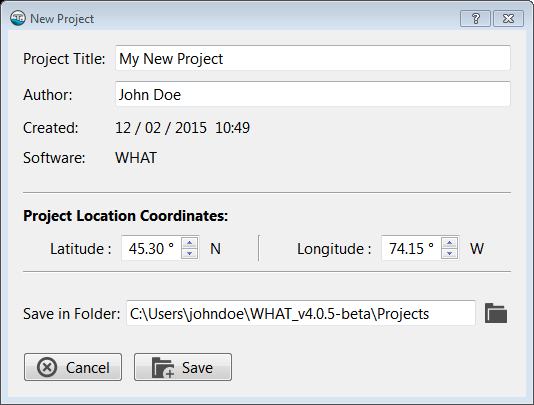
\includegraphics[width=0.5\textwidth]{WHAT_Screenshot_newproject}
\caption[New Project dialog window.]{New Project dialog window.}
\label{fig:new_proj_win}
\end{figure}

When a new project is saved, WHAT automatically creates within the project folder the predefined file organization that is presented in Figure~\ref{fig:proFolder_organization}.

\begin{figure}[h!]
\centering
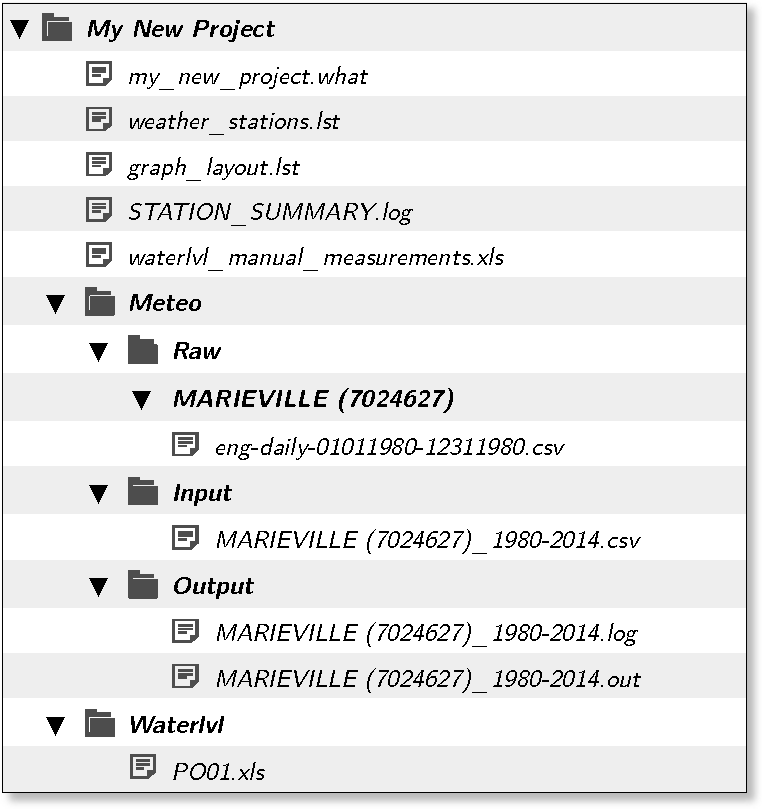
\includegraphics[width=0.5\textwidth]{file_and_folder_architecture}
\caption[Project folder file organization.]{Project folder file organization.}
\label{fig:proFolder_organization}
\end{figure}

In this example, we have the project My New Project, that is located within the folder Projects within the folder that contain the program.


\end{document}